% Created 2022-09-12 lun 10:03
% Intended LaTeX compiler: pdflatex
\documentclass[12pt]{article}
\usepackage[utf8]{inputenc}
\usepackage[T1]{fontenc}
\usepackage{graphicx}
\usepackage{grffile}
\usepackage{longtable}
\usepackage{wrapfig}
\usepackage{rotating}
\usepackage[normalem]{ulem}
\usepackage{amsmath}
\usepackage{textcomp}
\usepackage{amssymb}
\usepackage{capt-of}
\usepackage{hyperref}
\usepackage[spanish]{babel}
\usepackage{graphicx,geometry}
\geometry{ a4paper, left=1in, right=1in, top=1in, bottom=1in }
\renewcommand\familydefault{\sfdefault}
\usepackage{sectsty}
\sectionfont{\normalfont\Large }
\subsectionfont{\normalfont\normalsize}
\usepackage{tabularx}
\usepackage{listings}
\lstdefinestyle{mystyle}{
numbers=left,
showspaces=false,
frame=leftline,
showspaces=false,
showstringspaces=false,
showtabs=false,
numberstyle=\tiny,
}
\lstset{
style=mystyle,
literate={á}{{\'a}}1
{é}{{\'e}}1
{í}{{\'{\i}}}1
{ó}{{\'o}}1
{ú}{{\'u}}1
{Á}{{\'A}}1
{É}{{\'E}}1
{Í}{{\'I}}1
{Ó}{{\'O}}1
{Ú}{{\'U}}1
{ü}{{\"u}}1
{Ü}{{\"U}}1
{ñ}{{\~n}}1
{Ñ}{{\~N}}1
{¿}{{?``}}1
{¡}{{!``}}1
}
\makeatletter
\usepackage{fancyhdr}
\pagestyle{fancy}
\usepackage{mdframed}
\BeforeBeginEnvironment{minted}{\begin{mdframed}}
\AfterEndEnvironment{minted}{\end{mdframed}}
\author{Luis Eduardo Galindo Amaya (1274895)}
\date{2022-09-11}
\title{Listas Ligadas Sencillas}
\hypersetup{
 pdfauthor={Luis Eduardo Galindo Amaya (1274895)},
 pdftitle={Listas Ligadas Sencillas},
 pdfkeywords={},
 pdfsubject={},
 pdfcreator={Emacs 26.3 (Org mode 9.1.9)}, 
 pdflang={Spanish}}
\begin{document}


\newcommand{\docente}{Itzel Barriba Cazares}
\newcommand{\asignatura}{Estructuras de Datos (341)}
\newcommand{\semestre}{2022-2}

\newcommand{\miportada}[1]{
	\begin{titlepage}
		\vspace*{0.75in}
		\begin{flushleft}
			\sffamily
			\large #1       \\
			\Huge 
            \@title         \\
			\hrulefill
			\vspace{0.25in} \\
			\Large \@author \\
			\vspace*{\fill}
            
\includegraphics[width=\textwidth]{../includes/filler.png} \\
			\vspace*{\fill}
			\large
			\begin{tabular}{|l|l|}
              \hline
			  Asignatura & \asignatura \\
			  Docente    & \docente    \\
			  Fecha      & \@date      \\
              \hline
			\end{tabular}
		\end{flushleft}
	\end{titlepage}
}

\miportada{ Practica }

\fancyhf{}
\lhead{ \asignatura }
\rhead{ \semestre }
\rfoot{Página \thepage}

\setlength\parindent{0pt}   % eliminar el intentado
\setlength{\parskip}{1.2em}

\maketitle
\end{center}

\section*{Prodecimieto}
\label{sec:org2a05a66}
Se analizaron los documentos enviados por la profesora y se usaron como base para crear una libreria nueva para manejar lista ssencillas. La lista original simplemente ordenaba los elementos de menor a menor, en la nueva lista los terminos se pueden agregar por pocision:

\begin{itemize}
\item 0. Al inicio
\item -1. Al final
\item y cualquier otra pocision definida por el usuario.
\end{itemize}

\section*{Analisis del resultado}
\label{sec:orgaacce24}
Los resultados son los esperados, se pudo siplificar los metodos y ahora son mas legibles por si es necesario hacer modificaciones en el futuro

\section*{Capturas de Pantalla}
\label{sec:orgb7bb42c}
\subsection*{Inserción de datos}
\label{sec:orgbb16d73}
\begin{center}
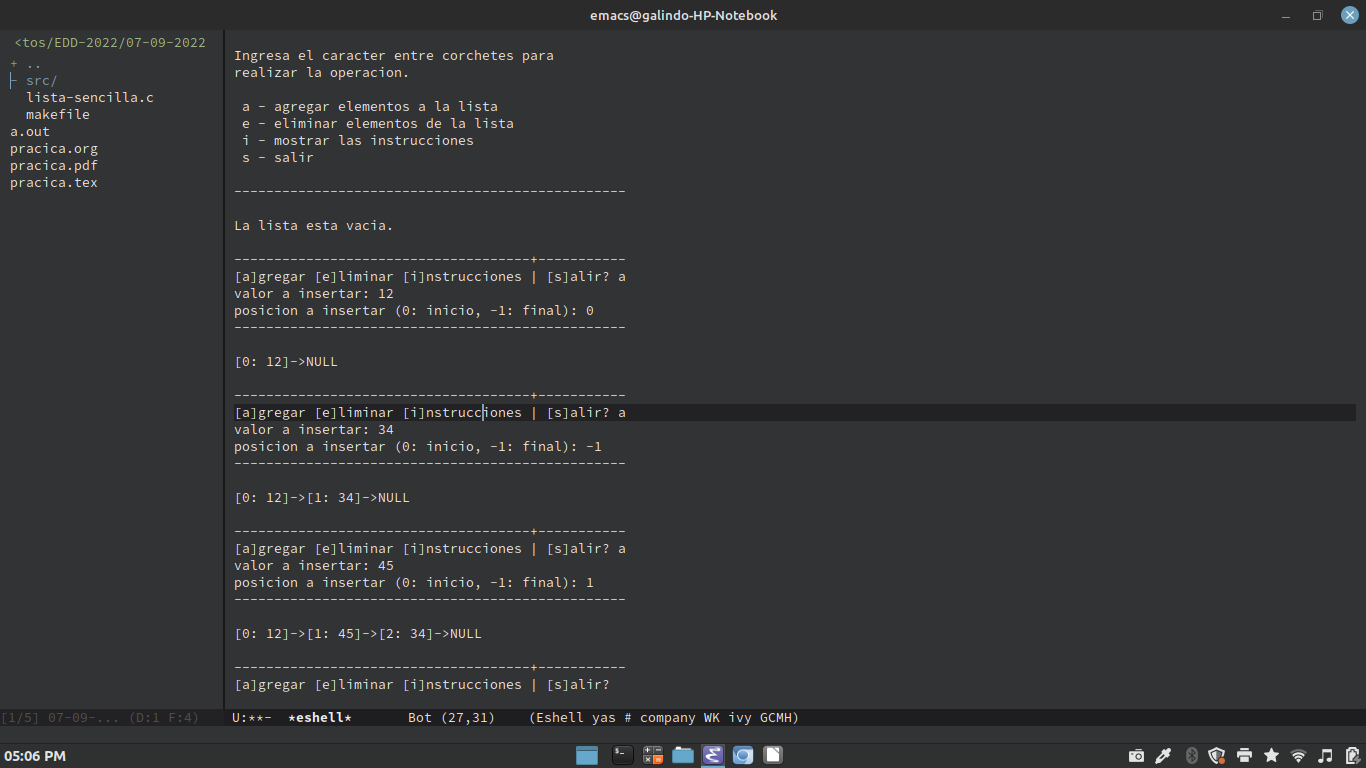
\includegraphics[width=.9\linewidth]{img/insertar.png}
\end{center}

\subsection*{Eliminación de datos}
\label{sec:orgb4d62ff}
\begin{center}
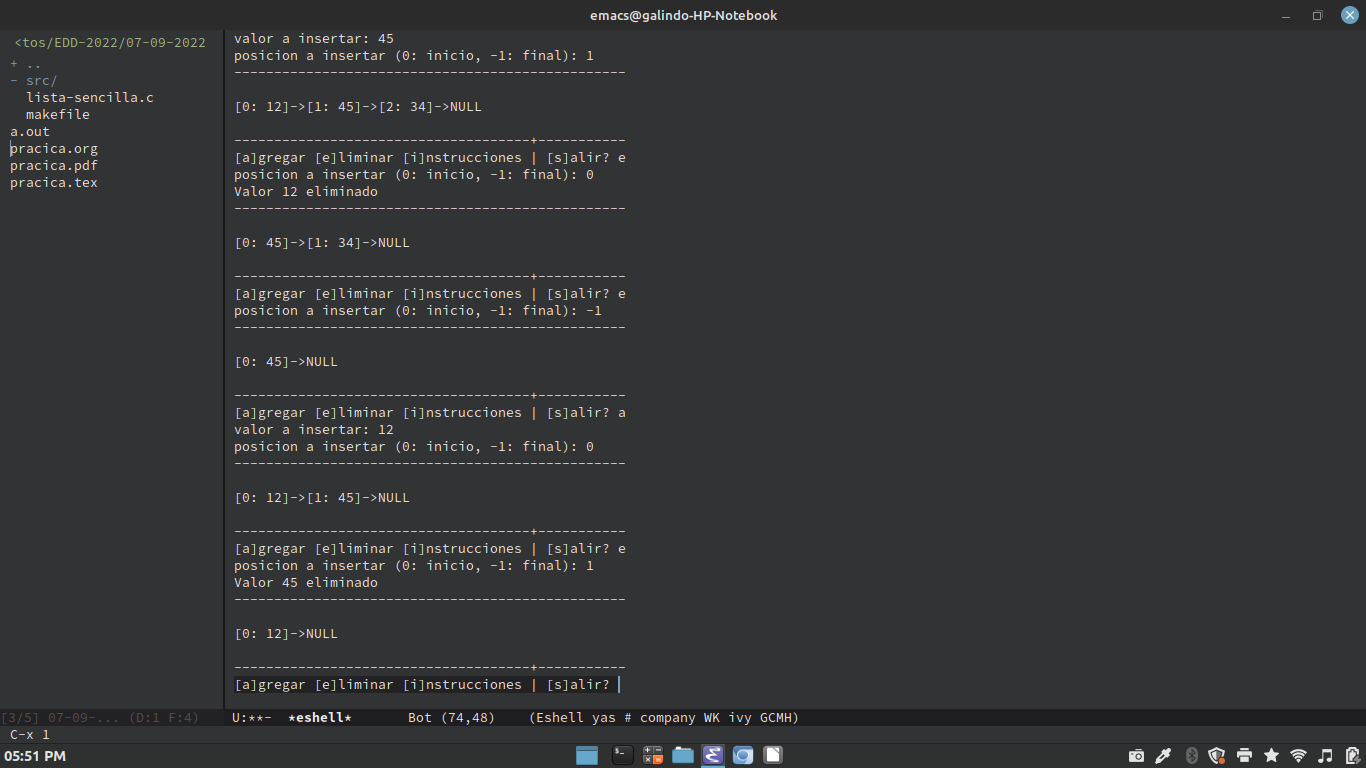
\includegraphics[width=.9\linewidth]{img/eliminar.png}
\end{center}

\section*{Conclusiones}
\label{sec:orgd3103d0}
Las listas a pesar de tener un comportamiento bien definido pueden modificarse para cumplir con roles muy específicos para la aplicación que se desea crear. 

\section*{Código}
\label{sec:org666220a}
\lstinputlisting{src/lista-sencilla.c}
\end{document}
